\subsection{Tool-Flow}
\begin{figure}
\centering
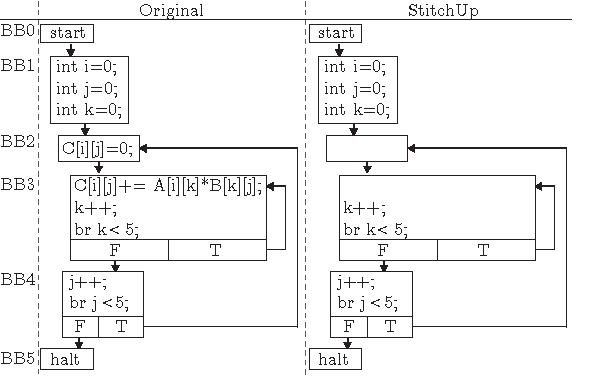
\includegraphics[width=3.5in]{./imgs/mmm_cdfg.pdf}
\caption{Control-Data-Flow Diagram for Matrix Multiplication example}
\label{fig:mmm_cdfg}
\end{figure}

What are the more concrete steps involved in getting this done?
What does the frontend look like (overview) and what about the backend,
is that mostly LegUp?

\begin{figure}
\centering
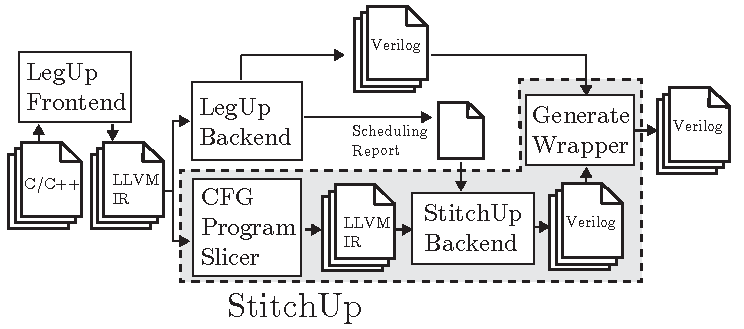
\includegraphics[width=3.5in]{./imgs/tool-flow.pdf}
\caption{Tool Flow Overview diagram}
\label{fig:tool_flow_diagram}
\end{figure}



\begin{figure*}[!t]
\centering
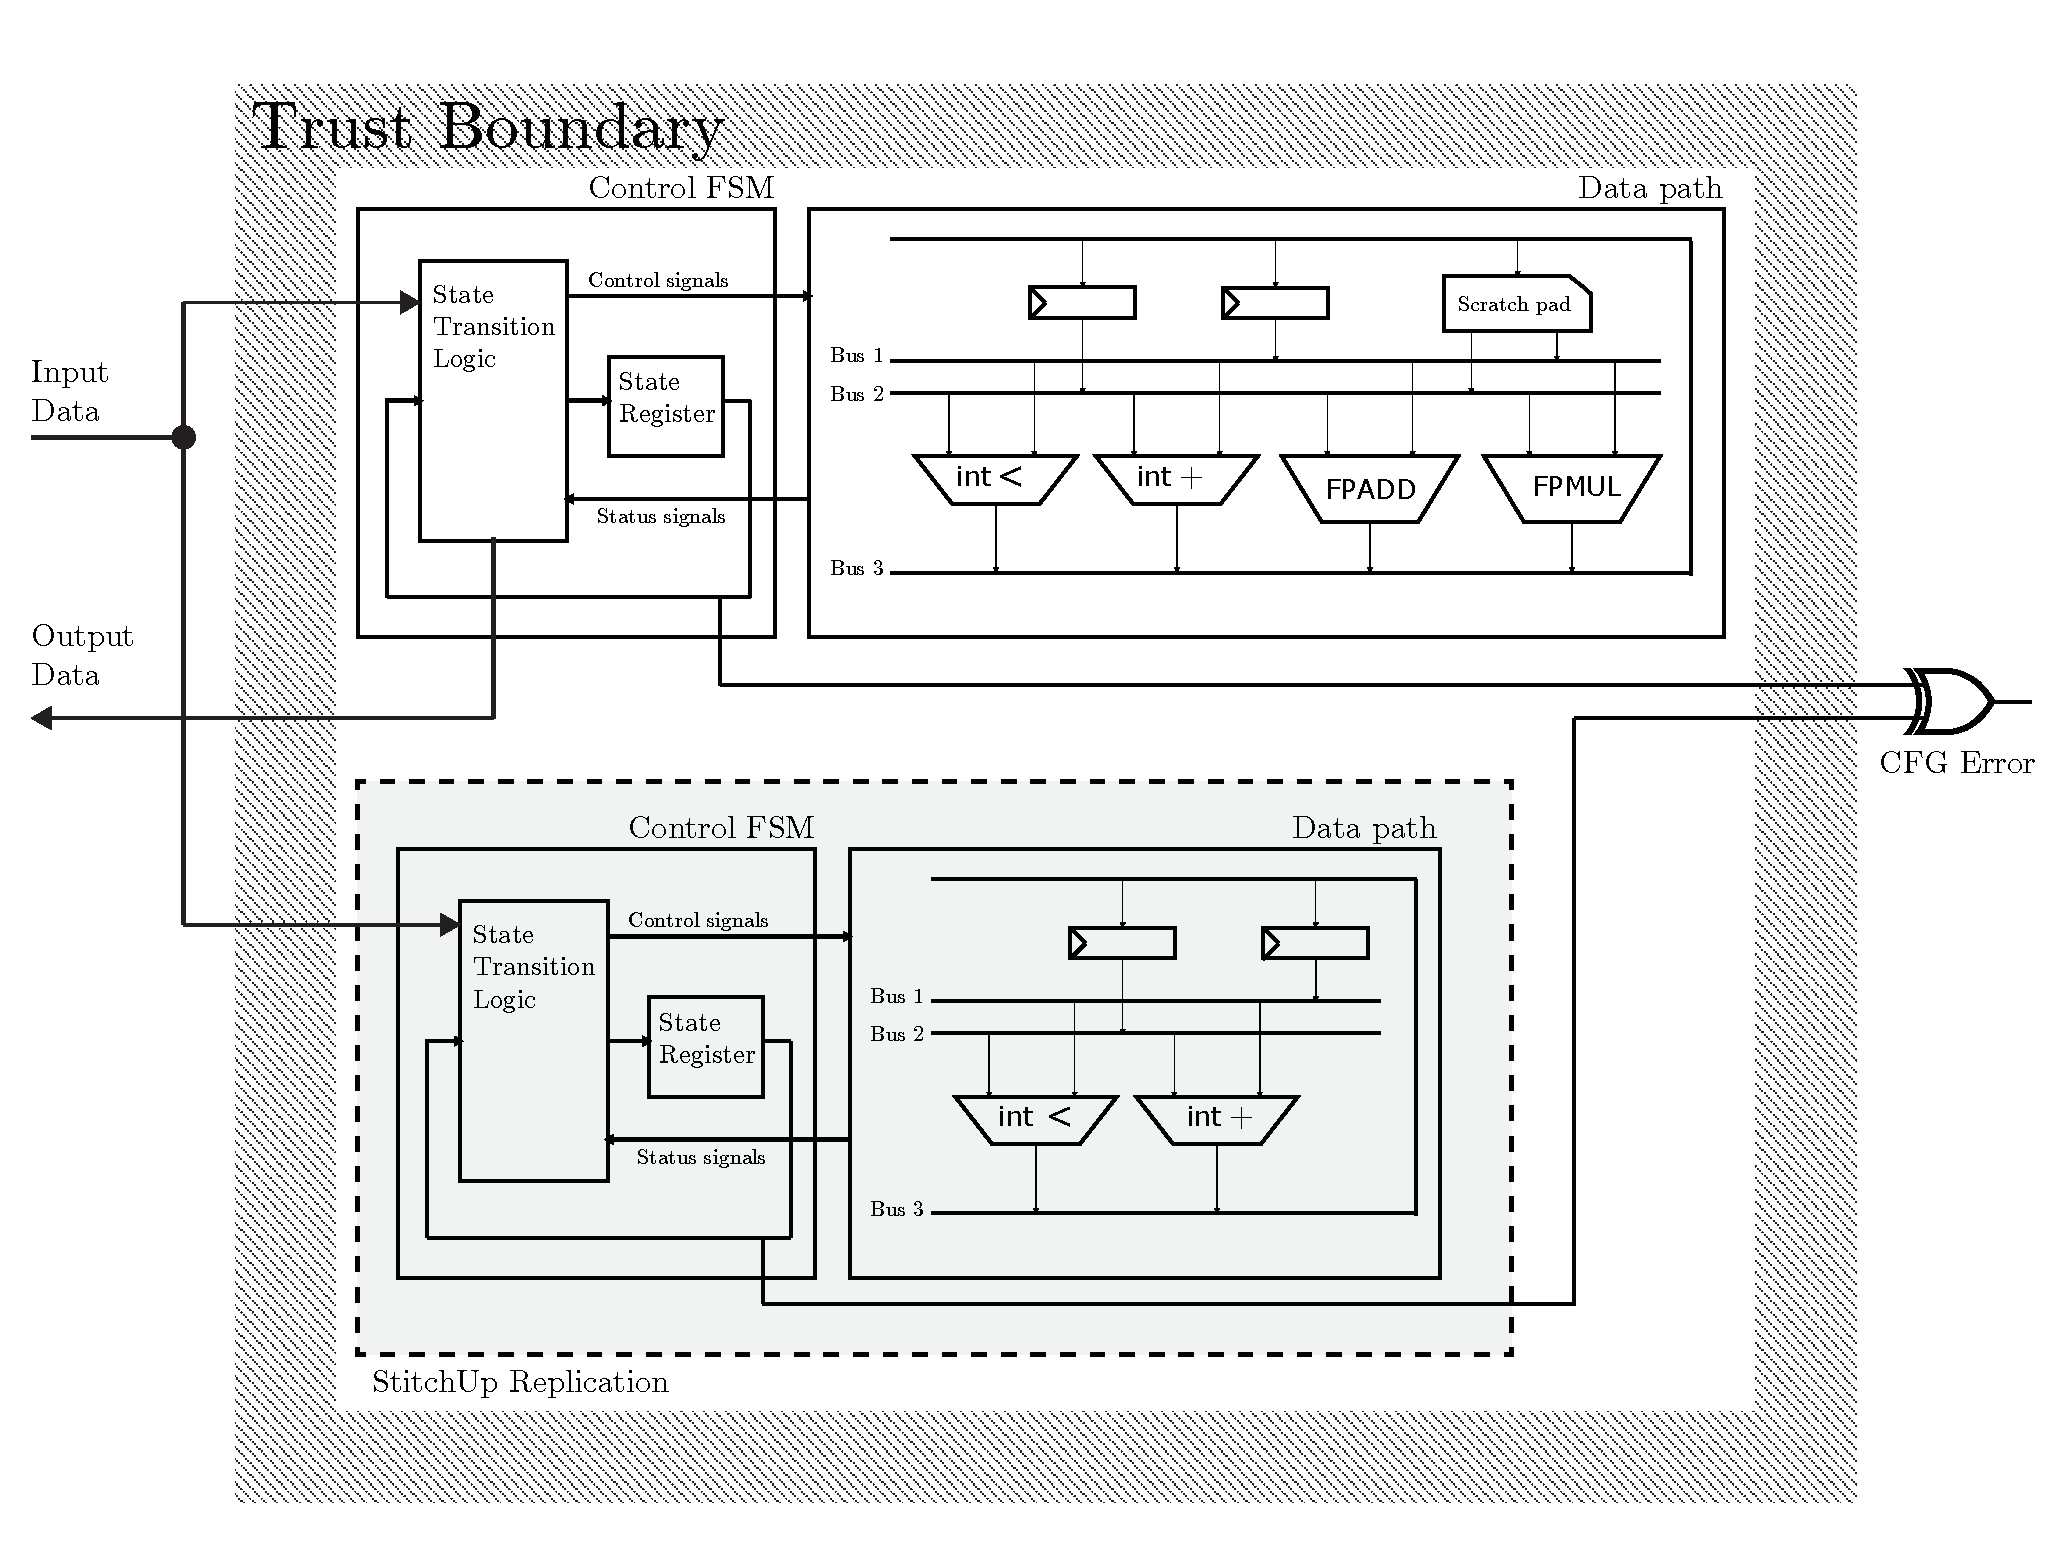
\includegraphics[width=7in]{./imgs/HLSArch.pdf}
\caption{StitchUp Replication for the Matrix Multiplication example, with Trust Boundary}
\label{fig:HLSArch}
\end{figure*}

